\documentclass[border=4pt]{standalone}
\usepackage{tikz}
\usetikzlibrary{positioning, arrows.meta, shapes.geometric, calc, fit, backgrounds, decorations.pathreplacing}
\usepackage{amsmath,amssymb}
\usepackage{soul}
\begin{document}
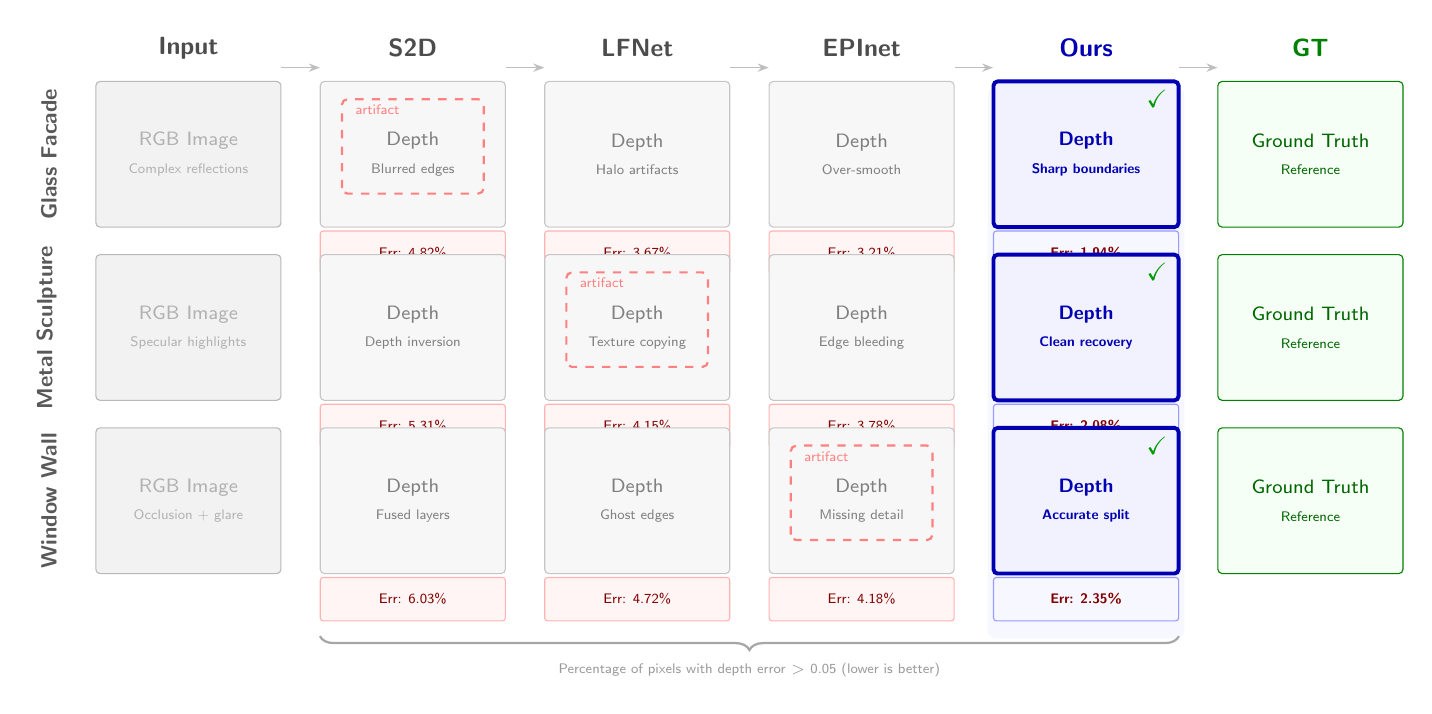
\begin{tikzpicture}[
    % --- Image placeholder box ---
    imgbox/.style={
        draw=gray!45, rounded corners=1.5pt,
        minimum width=2.35cm, minimum height=1.85cm,
        inner sep=0pt, align=center,
        font=\sffamily\scriptsize, text=black!50,
        fill=gray!6,
    },
    % --- "Ours" highlighted box ---
    oursbox/.style={
        imgbox,
        draw=blue!70!black, line width=1.4pt,
        fill=blue!5,
        font=\sffamily\scriptsize\bfseries, text=blue!70!black,
    },
    % --- GT box ---
    gtbox/.style={
        imgbox,
        fill=green!4, draw=green!50!black,
        font=\sffamily\scriptsize, text=green!40!black,
    },
    % --- Input box ---
    inputbox/.style={
        imgbox,
        fill=gray!10, draw=gray!55,
        font=\sffamily\scriptsize, text=gray!60,
    },
    % --- Error map box ---
    errbox/.style={
        draw=red!30, rounded corners=1pt,
        minimum width=2.35cm, minimum height=0.55cm,
        inner sep=0pt, align=center,
        font=\sffamily\tiny, text=red!50!black,
        fill=red!4,
    },
    % --- Column header ---
    colhead/.style={
        font=\sffamily\small\bfseries, text=black!70, align=center,
    },
    % --- Scene label ---
    scenelbl/.style={
        font=\sffamily\footnotesize\bfseries, text=black!65,
    },
    % --- Arrow between columns ---
    flowarr/.style={
        -{Stealth[length=4pt]}, color=black!25, thin,
    },
    % --- Brace for scene grouping ---
    brace/.style={
        decorate, decoration={brace, amplitude=5pt, mirror},
        thick, black!35,
    },
    % --- Error value label ---
    errval/.style={
        font=\sffamily\tiny, text=black!45,
    },
]

% ============================================================
% Column x-positions
% ============================================================
\def\cola{0}
\def\colb{2.85}
\def\colc{5.70}
\def\cold{8.55}
\def\cole{11.40}
\def\colf{14.25}

% Column headers
\node[colhead] at (\cola,  2.25) {Input};
\node[colhead] at (\colb,  2.25) {S2D};
\node[colhead] at (\colc,  2.25) {LFNet};
\node[colhead] at (\cold,  2.25) {EPInet};
\node[colhead, text=blue!70!black] at (\cole, 2.25) {Ours};
\node[colhead, text=green!50!black] at (\colf, 2.25) {GT};

% ============================================================
% Row y-positions
% ============================================================
\def\rowA{0.9}
\def\rowB{-1.3}
\def\rowC{-3.5}

% ============================================================
% Scene 1 — Glass Facade (non-Lambertian challenge)
% ============================================================
\node[scenelbl, rotate=90, anchor=south] at (-1.55, \rowA) {Glass Facade};

\node[inputbox] (s1input) at (\cola, \rowA)
    {RGB Image\\[2pt]{\tiny Complex reflections}};
\node[imgbox] (s1s2d) at (\colb, \rowA)
    {Depth\\[2pt]{\tiny Blurred edges}};
\node[imgbox] (s1lf) at (\colc, \rowA)
    {Depth\\[2pt]{\tiny Halo artifacts}};
\node[imgbox] (s1epi) at (\cold, \rowA)
    {Depth\\[2pt]{\tiny Over-smooth}};
\node[oursbox] (s1ours) at (\cole, \rowA)
    {Depth\\[2pt]{\tiny Sharp boundaries}};
\node[gtbox] (s1gt) at (\colf, \rowA)
    {Ground Truth\\[2pt]{\tiny Reference}};

% Error bars row 1
\node[errbox] at (\colb, \rowA-1.25) {Err: 4.82\%};
\node[errbox] at (\colc, \rowA-1.25) {Err: 3.67\%};
\node[errbox] at (\cold, \rowA-1.25) {Err: 3.21\%};
\node[errbox, draw=blue!40, fill=blue!3] at (\cole, \rowA-1.25) {\textbf{Err: 1.94\%}};

% ============================================================
% Scene 2 — Metal Sculpture (specular challenge)
% ============================================================
\node[scenelbl, rotate=90, anchor=south] at (-1.55, \rowB) {Metal Sculpture};

\node[inputbox] (s2input) at (\cola, \rowB)
    {RGB Image\\[2pt]{\tiny Specular highlights}};
\node[imgbox] (s2s2d) at (\colb, \rowB)
    {Depth\\[2pt]{\tiny Depth inversion}};
\node[imgbox] (s2lf) at (\colc, \rowB)
    {Depth\\[2pt]{\tiny Texture copying}};
\node[imgbox] (s2epi) at (\cold, \rowB)
    {Depth\\[2pt]{\tiny Edge bleeding}};
\node[oursbox] (s2ours) at (\cole, \rowB)
    {Depth\\[2pt]{\tiny Clean recovery}};
\node[gtbox] (s2gt) at (\colf, \rowB)
    {Ground Truth\\[2pt]{\tiny Reference}};

% Error bars row 2
\node[errbox] at (\colb, \rowB-1.25) {Err: 5.31\%};
\node[errbox] at (\colc, \rowB-1.25) {Err: 4.15\%};
\node[errbox] at (\cold, \rowB-1.25) {Err: 3.78\%};
\node[errbox, draw=blue!40, fill=blue!3] at (\cole, \rowB-1.25) {\textbf{Err: 2.08\%}};

% ============================================================
% Scene 3 — Mixed Window/Wall (occlusion + reflection)
% ============================================================
\node[scenelbl, rotate=90, anchor=south] at (-1.55, \rowC) {Window Wall};

\node[inputbox] (s3input) at (\cola, \rowC)
    {RGB Image\\[2pt]{\tiny Occlusion + glare}};
\node[imgbox] (s3s2d) at (\colb, \rowC)
    {Depth\\[2pt]{\tiny Fused layers}};
\node[imgbox] (s3lf) at (\colc, \rowC)
    {Depth\\[2pt]{\tiny Ghost edges}};
\node[imgbox] (s3epi) at (\cold, \rowC)
    {Depth\\[2pt]{\tiny Missing detail}};
\node[oursbox] (s3ours) at (\cole, \rowC)
    {Depth\\[2pt]{\tiny Accurate split}};
\node[gtbox] (s3gt) at (\colf, \rowC)
    {Ground Truth\\[2pt]{\tiny Reference}};

% Error bars row 3
\node[errbox] at (\colb, \rowC-1.25) {Err: 6.03\%};
\node[errbox] at (\colc, \rowC-1.25) {Err: 4.72\%};
\node[errbox] at (\cold, \rowC-1.25) {Err: 4.18\%};
\node[errbox, draw=blue!40, fill=blue!3] at (\cole, \rowC-1.25) {\textbf{Err: 2.35\%}};

% ============================================================
% Flow arrows — top row only (indicates processing direction)
% ============================================================
\foreach \c/\d in {\cola/\colb, \colb/\colc, \colc/\cold, \cold/\cole, \cole/\colf}{
    \draw[flowarr] (\c+1.18, 2.0) -- (\d-1.18, 2.0);
}

% ============================================================
% Highlight region — "Ours" column background accent
% ============================================================
\begin{scope}[on background layer]
    \fill[blue!3, rounded corners=3pt]
        (\cole-1.25, 1.75) rectangle (\cole+1.25, \rowC-1.75);
\end{scope}

% ============================================================
% Bottom annotation brace — Best viewed with error maps
% ============================================================
\draw[brace] (\colb-1.18, \rowC-1.72) -- (\cole+1.18, \rowC-1.72)
    node[midway, below=6pt, font=\sffamily\tiny, text=black!40]
    {Percentage of pixels with depth error $>$ 0.05 (lower is better)};

% ============================================================
% Red dashed region marking artifact area (Scene 1, methods)
% ============================================================
\draw[red!50, dashed, thick, rounded corners=2pt]
    (\colb-0.9, \rowA-0.5) rectangle (\colb+0.9, \rowA+0.7);
\node[font=\sffamily\tiny, text=red!50, anchor=north west]
    at (\colb-0.85, \rowA+0.75) {artifact};

\draw[red!50, dashed, thick, rounded corners=2pt]
    (\colc-0.9, \rowB-0.5) rectangle (\colc+0.9, \rowB+0.7);
\node[font=\sffamily\tiny, text=red!50, anchor=north west]
    at (\colc-0.85, \rowB+0.75) {artifact};

\draw[red!50, dashed, thick, rounded corners=2pt]
    (\cold-0.9, \rowC-0.5) rectangle (\cold+0.9, \rowC+0.7);
\node[font=\sffamily\tiny, text=red!50, anchor=north west]
    at (\cold-0.85, \rowC+0.75) {artifact};

% ============================================================
% Green checkmark on Ours results
% ============================================================
\node[font=\small, text=green!60!black] at (\cole+0.9, \rowA+0.7) {$\checkmark$};
\node[font=\small, text=green!60!black] at (\cole+0.9, \rowB+0.7) {$\checkmark$};
\node[font=\small, text=green!60!black] at (\cole+0.9, \rowC+0.7) {$\checkmark$};

\end{tikzpicture}
\end{document}